%%%%%%%%%%%%%%%%%%%%%%%%%%%%%%%%%%%%%
% This is a template file for trying to make boxes, minipages, etc.

\documentclass[pagesize=auto]{scrbook}

\usepackage[english]{babel}

\usepackage{comment}
\usepackage{graphicx}
\usepackage{hyperref}
\usepackage{wrapfig}
\usepackage{xspace}
\usepackage{xcolor}


% This file is for commands / macros / functions. 

% These are useful because HTML output corrupts the result of the \latex command.
\newcommand{\latex}{LaTeX\xspace}
\newcommand{\tex}{TeX\xspace}

\newcommand\nextpage[1][]{
\ifdefined\HCode {
  \HCode{<mbp:pagebreak />}}
\else
  \newpage
\fi
}

% Wrapfigure doesn't typeset well in the ebook conversion! 
% marginal Boxes for special interest points
\definecolor{grey}{gray}{0.96}
% simple definition rather than newenvironment because of problems
% nesting parbox
\def\BOX#1#2{
  \begin{wrapfigure}{r}{2.5cm}
  \colorbox{grey}{\parbox{2cm}{
  % title
  \flushleft #1 \\
  \vspace*{0.1in}
  \small
  % paragraph text
  #2}   
  }
  \end{wrapfigure}
}



\begin{document}

Hello outside a box!

\begin{center}
Hello outside a box, centered!
\fbox{Hello in a box, centered!}
\end{center}

\begin{figure}
  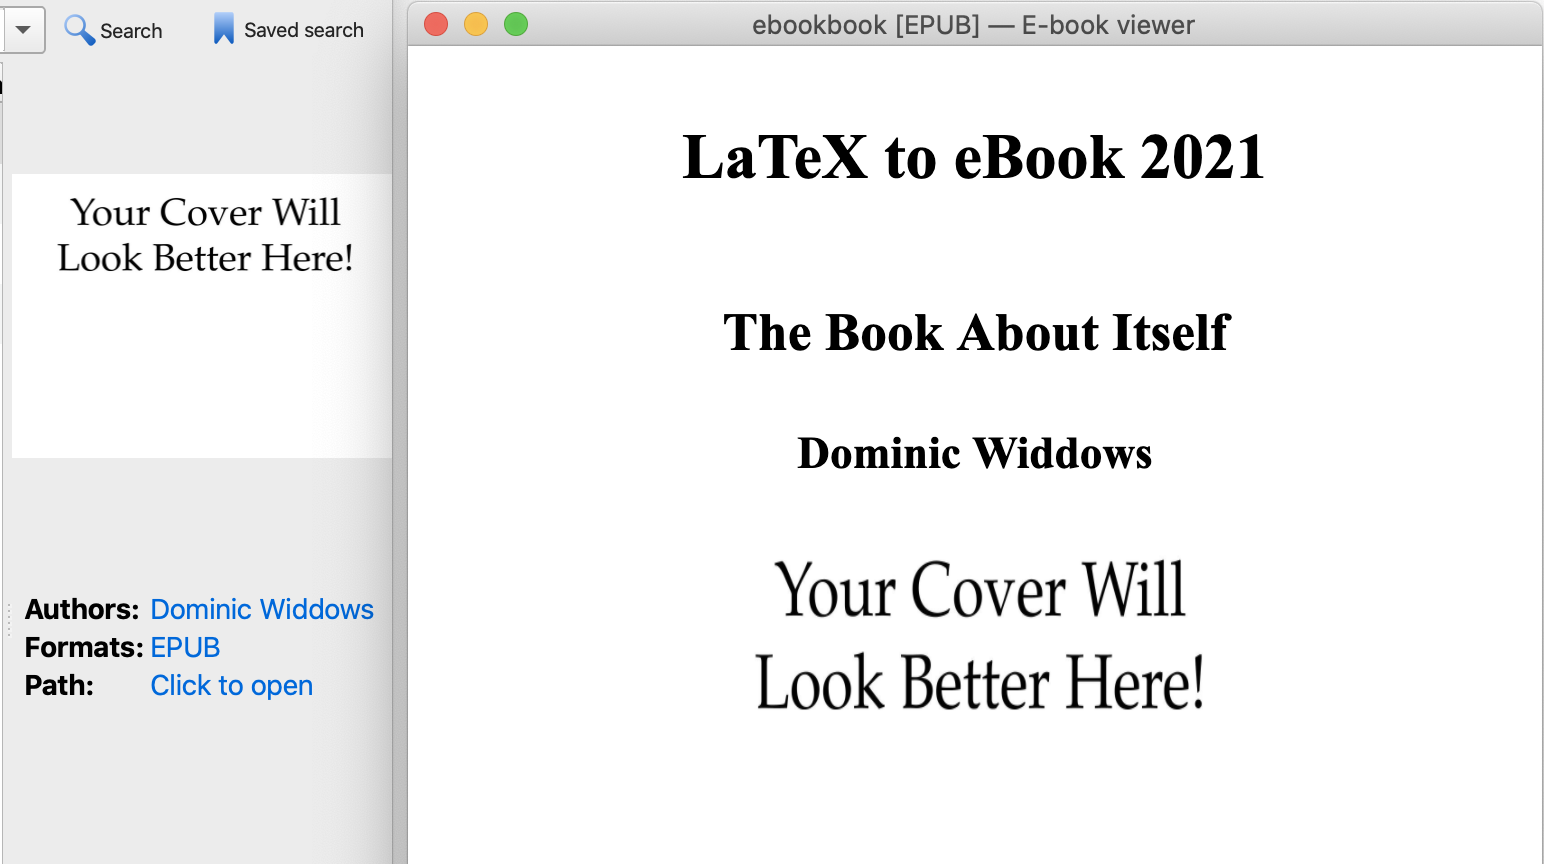
\includegraphics[width=0.5\linewidth]{../../images/calibre_screenshot.png}
  \caption{Screenshot in a figure but not a box}
\end{figure}

\begin{center}
\begin{figure}
  \begin{center}
  \fbox{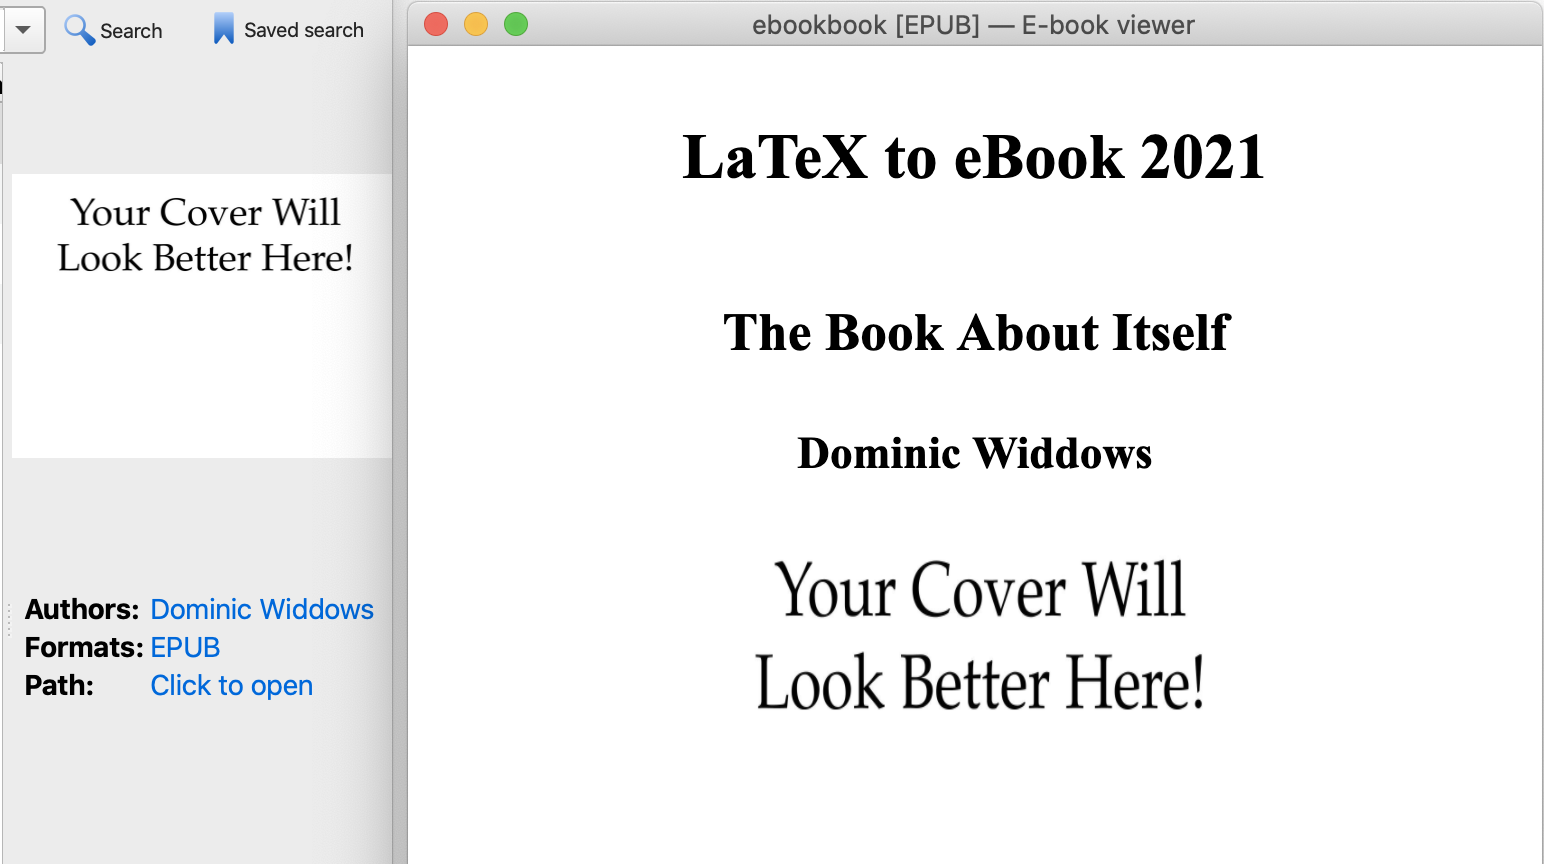
\includegraphics[width=0.5\linewidth]{../../images/calibre_screenshot.png}}
  \caption{Screenshot in an fbox in a figure - floats to the left, however often I try to center it}
  \end{center}
\end{figure}
\end{center}

\begin{figure}
    \begin{minipage}{0.6\textwidth}
        \makebox[0.4\columnwidth][l]{line1}
        \par
        \makebox[0.4\columnwidth][l]{line2}
        \par
        \makebox[0.4\columnwidth][r]{line3}
    \end{minipage}
    \begin{minipage}{0.375\textwidth}
        \centering 
        %\includegraphics{pic.jpg}
        image
    \end{minipage}
\end{figure}

So what's the problem?

\end{document}
